\section{Using Azure ML API/ SDK/ CLI}
\subsection{Introduction}
The \gls{g_Python} \gls{AMLSDKv2} with the package library
\begin{center}
	\textbf{azure-ai-ml}
\end{center}
and the \gls{AMLSDKv1} with 
\begin{center}
	\textbf{azureml-core}
\end{center}
are \gls{API}s for the \gls{AML} workspace and it's services. The \gls{CLI} package for \gls{AML} contains a more compact command line style workflows, that need to be executed. The format in v2 is normally \textit{<noun><verb><option>}.\\

The \gls{SDK} is more directed to the development, while the \gls{CLI} is more convient for a \gls{CI}/\gls{CD} process. The later is due to the more compact way of executing commands.\footnote{Reference: \href{https://learn.microsoft.com/en-us/answers/questions/1395777/what-is-the-difference-between-azure-ail-ml-and-az}{Difference CLI, SDK}, \href{https://github.com/microsoft/MLOps}{MLOps Python AML}
}
\subsection{Basics}

\subsubsection{Working with conda}
\paragraph{Interacting with conda from the terminal}
Here are three ways to interact with the python interpreter:
\begin{description}
	\item[conda comand] Starting the \textit{Anaconda Navigator} and start the \gls{IDE} from there. This then allows to interact with conda throug the \textbf{conda} \textbf{Cmdlet} from the terminal.

	\item[PowerShell Extension] If the local machine has some restriction, that prohibist the use of the command \textbf{conda} from the powershell terminal.
	\begin{figure}[H]
		\centering
		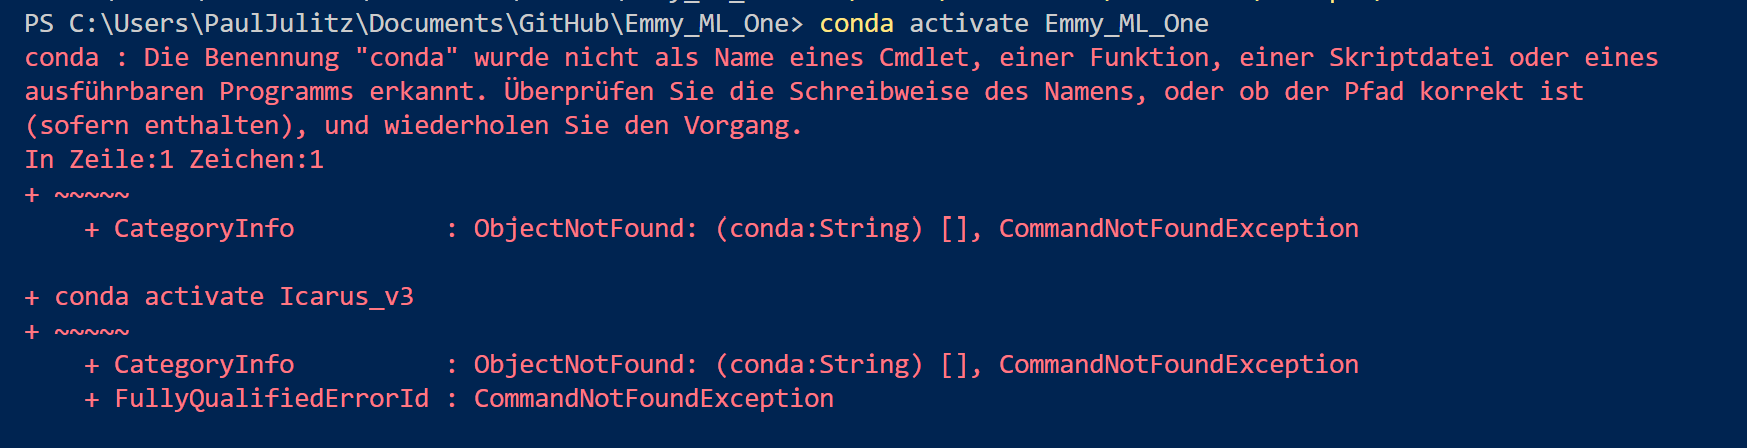
\includegraphics[scale = 0.3]{attachment/chapter_AML/Scc023}
		\caption{Terminal Response by using conda command}
	\end{figure}
	Still, the following powershell script allows when execute to use a \textit{powershell extension}, that bypass this problem.
	\begin{lstlisting}[style=CMD, caption={.ps1 script}, captionpos=b]
		#region conda initialize
		# !! Contents within this block are managed by 'conda init' !!
		$varPath  = "C:\User\" + (Get-ChildItem Env:USERNAME).Value + "\anaconda\Scripts\conda.exe"
		If (Test-Path $varPath ) {
			(& $varPath  "shell.powershell" "hook") | Out-String | ?{$_} | Invoke-Expression
		}
		#endregion
	\end{lstlisting}
	This powershell extension allows you with the \gls{g_conda} program.
	\begin{figure}[H]
		\centering
		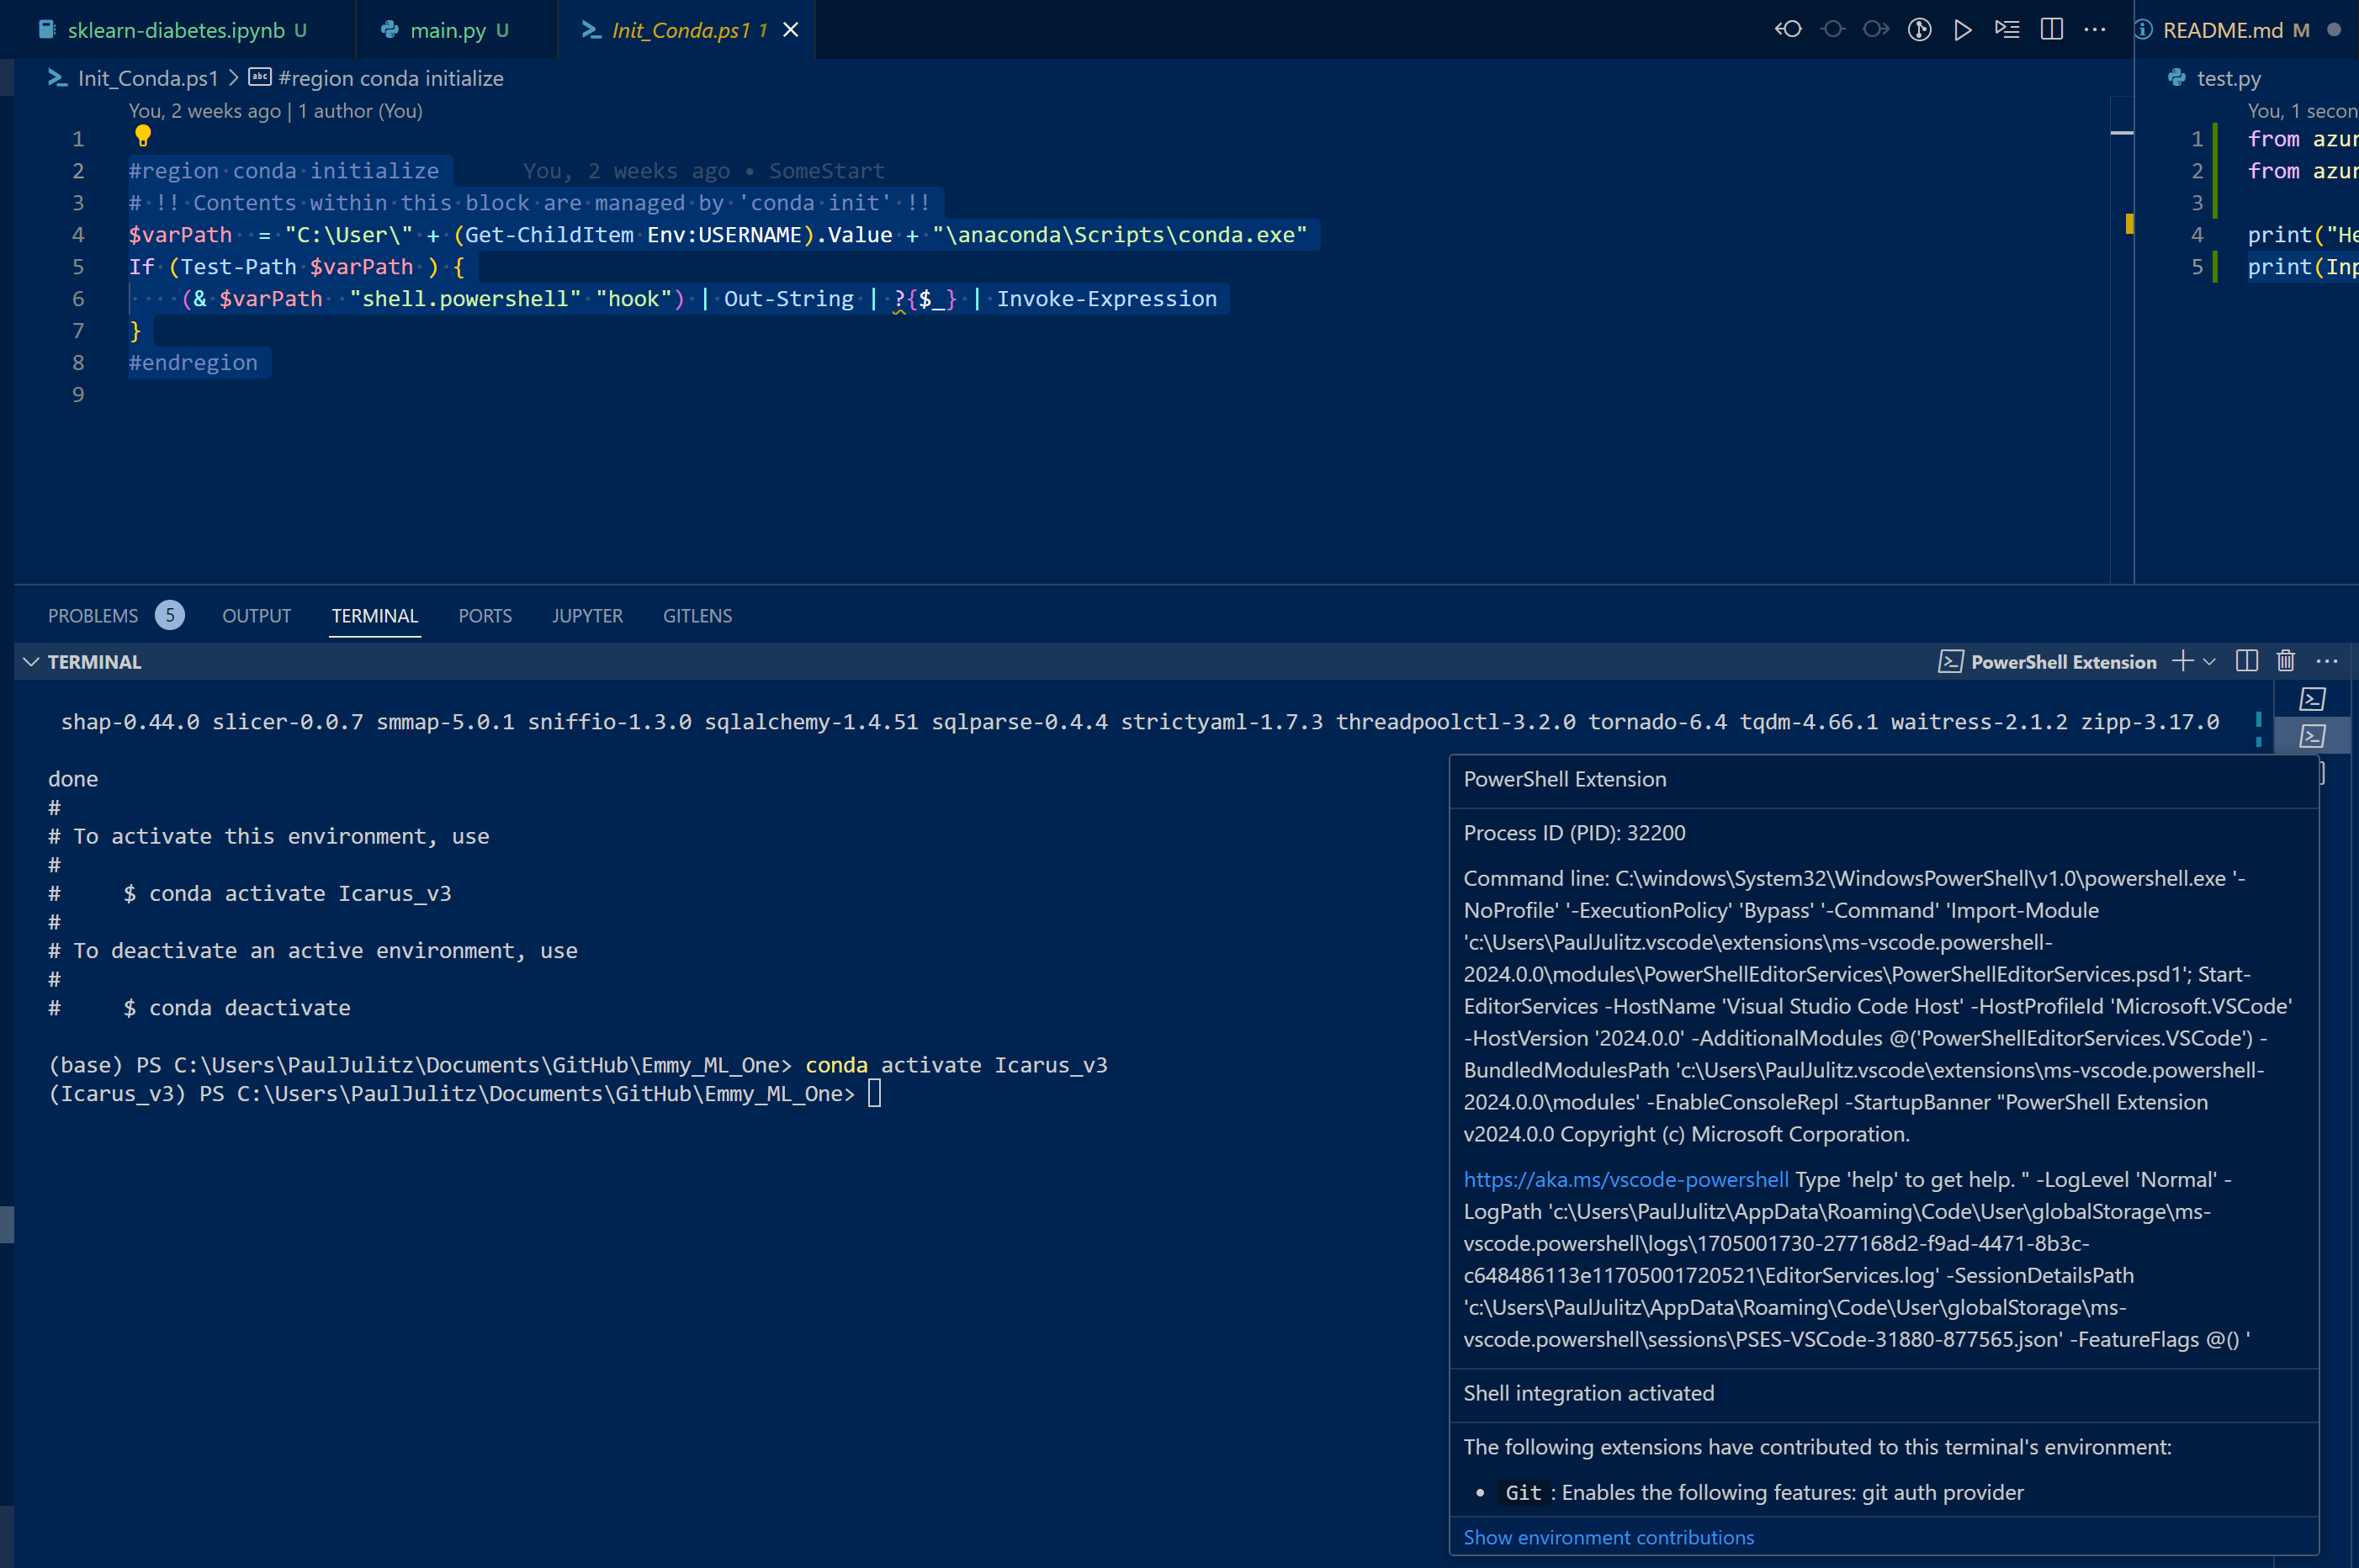
\includegraphics[scale = 0.2]{attachment/chapter_AML/Scc026}
		\caption{PowerShell Extension}
	\end{figure}
	One restriction still exists. In \gls{vsc} the option to run a program requires to create a python terminal in which the \textbf{conda} command can be access. This will not work, because a new terminal will be created in which the \textbf{conda} command can't be access. However, the python interpreter in a specific \gls{g_conda} \gls{VEN} can still be access by providing the direct path to it.
	\begin{figure}[H]
		\centering
		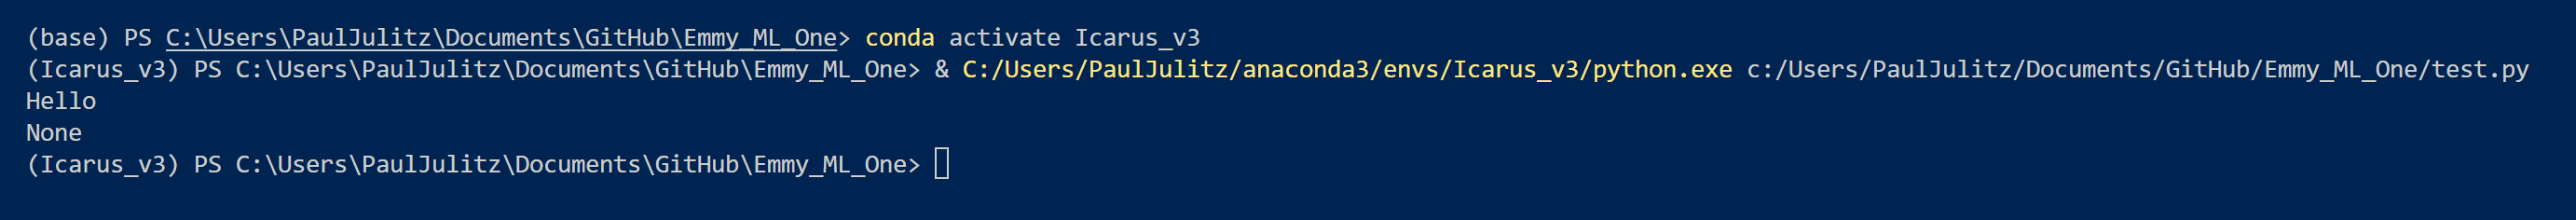
\includegraphics[scale = 0.4]{attachment/chapter_AML/Scc027}
		\caption{PowerShell Extension and Python Interpreter}
	\end{figure}
	\begin{lstlisting}[style=CMD, caption={Commands}, captionpos=b]
		(base) PS C:\Users\PaulJulitz\Documents\GitHub\Emmy_ML_One> conda activate Icarus_v3
		(Icarus_v3) PS C:\Users\PaulJulitz\Documents\GitHub\Emmy_ML_One> & C:/Users/PaulJulitz/anaconda3/envs/Icarus_v3/python.exe c:/Users/PaulJulitz/Documents/GitHub/Emmy_ML_One/test.py  
		Hello
		None
		(Icarus_v3) PS C:\Users\PaulJulitz\Documents\GitHub\Emmy_ML_One>
	\end{lstlisting}
	\item[Pointing to the interpreter] If the conda command can't be used.
	Then the python interpreter it self can be selected.
	\begin{figure}[H]
		\centering
		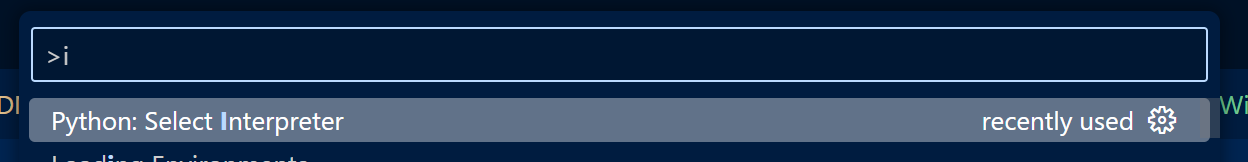
\includegraphics[scale = 0.4]{attachment/chapter_AML/Scc025}
		\caption{Selecting the python interpreter in \gls{vsc}}
	\end{figure}
	Running a python script will use the python interpreter inside the selected \gls{g_conda} \gls{VEN}.
	\begin{figure}[H]
		\centering
		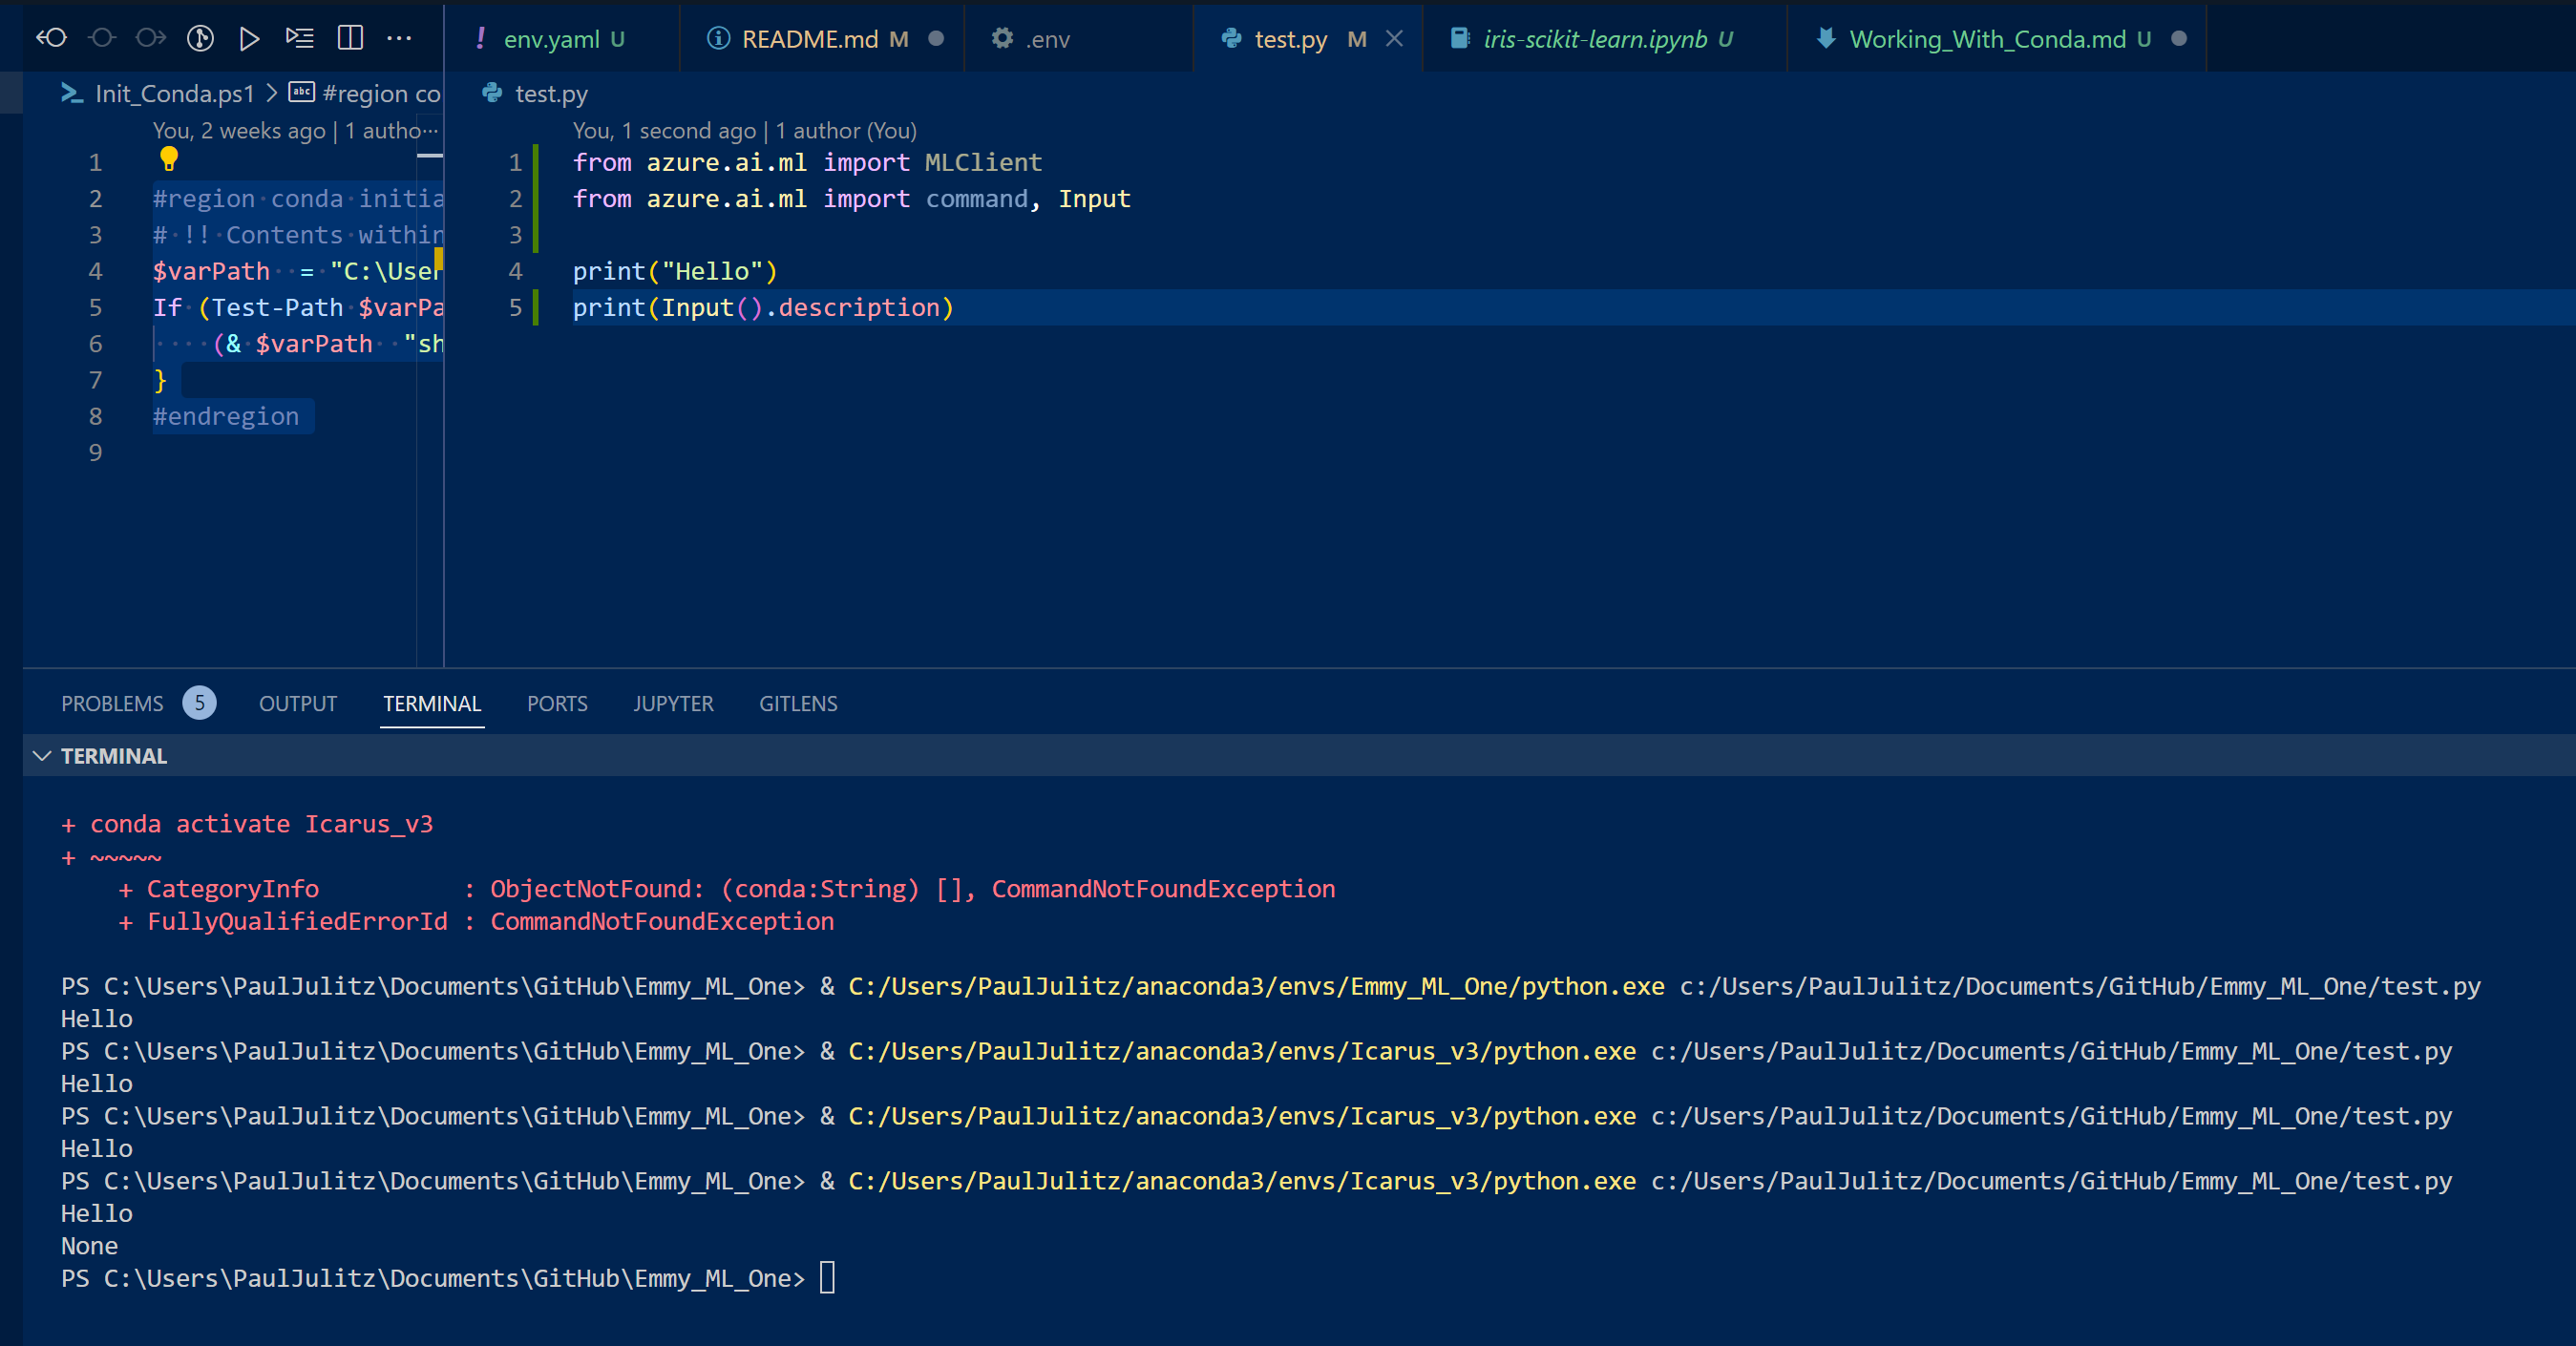
\includegraphics[scale = 0.2]{attachment/chapter_AML/Scc024}
		\caption{Terminal Response by using the python interpreter}
	\end{figure}
\end{description}

\begin{comment}
\subsubsection{*Example SDK/ CLI}
References: \href{https://learn.microsoft.com/de-de/azure/machine-learning/how-to-setup-vs-code?view=azureml-api-2}{Start Setup VS-Code}
\href{https://learn.microsoft.com/de-de/azure/machine-learning/how-to-launch-vs-code-remote?view=azureml-api-2&tabs=vscode-desktop}{Case: VSCode Desktop}
\href{https://learn.microsoft.com/de-de/azure/machine-learning/tutorial-train-deploy-image-classification-model-vscode?view=azureml-api-2}{Tutorial: Reference SDK/CLI v2 Example Doc}
\href{https://github.com/Azure/azureml-examples/blob/main/cli/jobs/single-step/tensorflow/mnist/src/train.py}{git Repo Example SDK/CLI v2}

\subsubsection{* Utilizing other ressources in Azure ML workspace}
With both Azure and Azure ML Extension it is possible to manage the resources directly. 
%How exaclty, I'll see.
\begin{figure}[H]
	\centering
	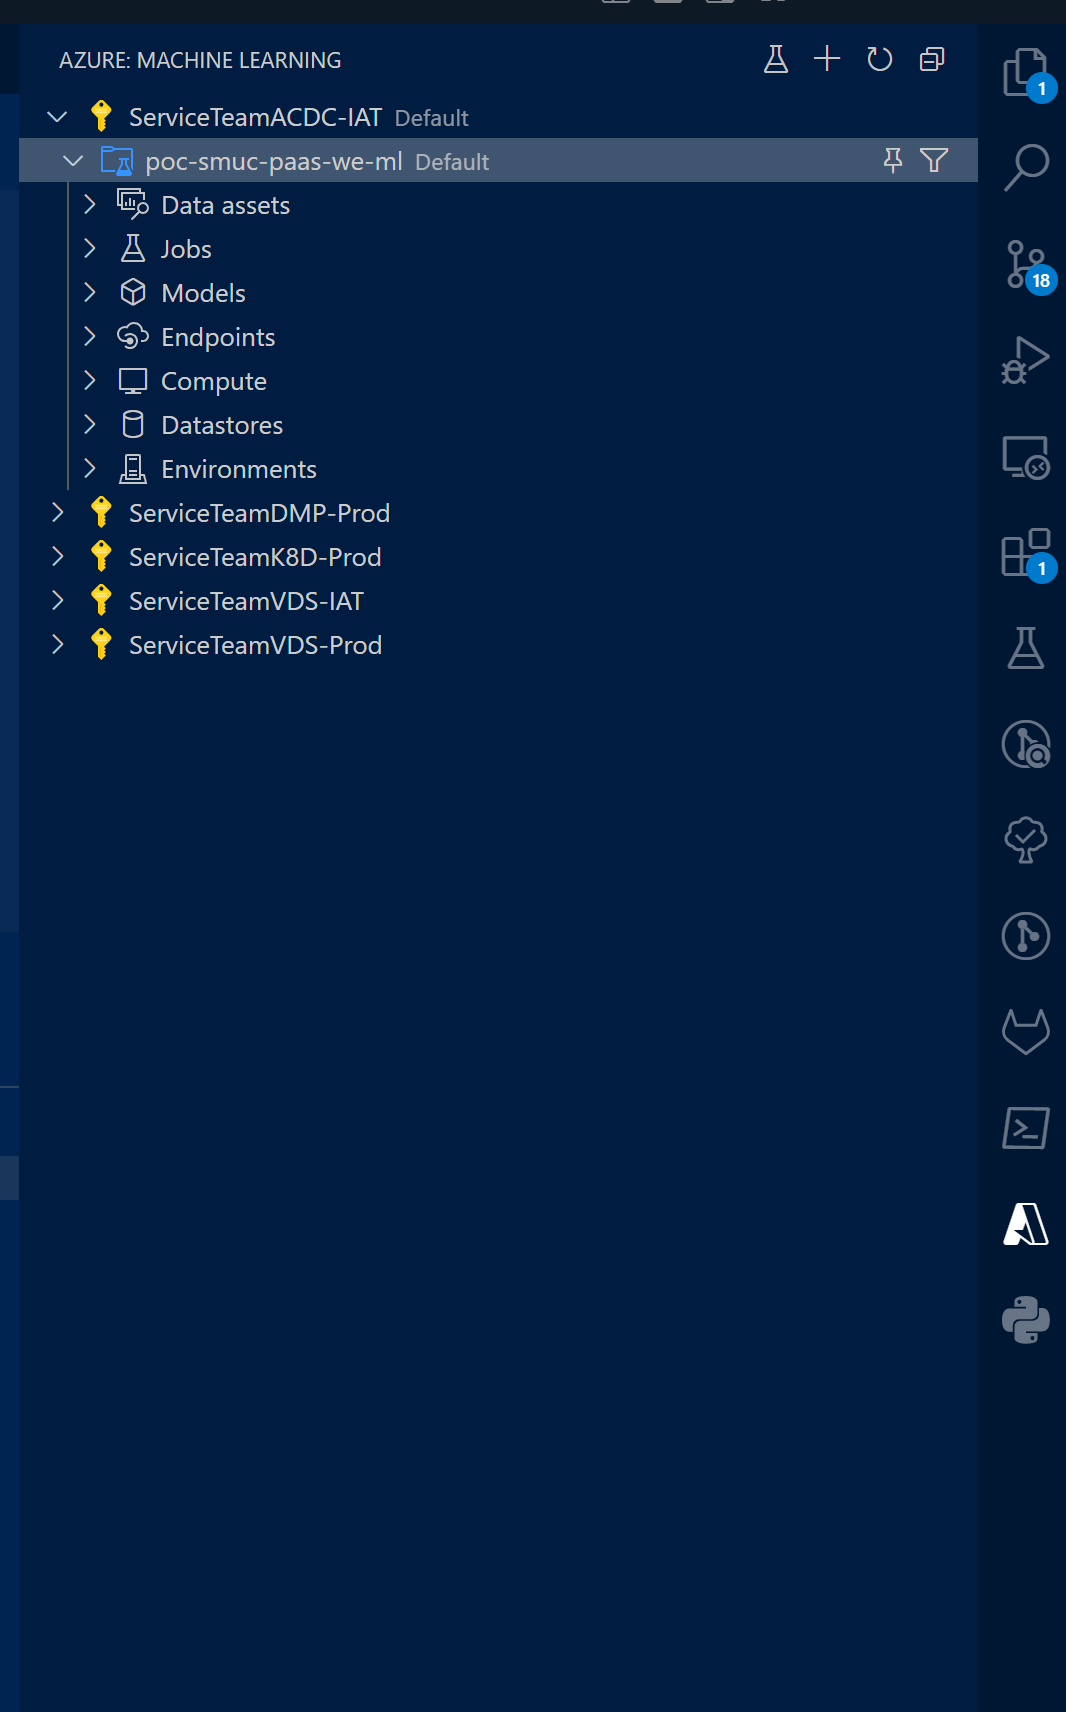
\includegraphics[scale = 0.3]{attachment/chapter_AML/Scc020}
	\caption{Azure and Azure ML Extension}
\end{figure}
\end{comment}



\subsection{Running ON the Compute Instance}
\subsubsection{Single Jupyter Notebook Connection}
Reference: \href{https://learn.microsoft.com/de-de/azure/machine-learning/how-to-launch-vs-code-remote?view=azureml-api-2&tabs=vscode-desktop}{Getting started with VS-Code Desktop}\\

With this functionality, any local \gls{g_JupyterNotebook} can use the a remote server connection to execute code on a compute instance with a \gls{g_Kernel_Jy}.\\

To run a \gls{g_JupyterNotebook}, a \gls{g_Kernel_Jy} needs to be selected.

\begin{figure}[H]
	\centering
	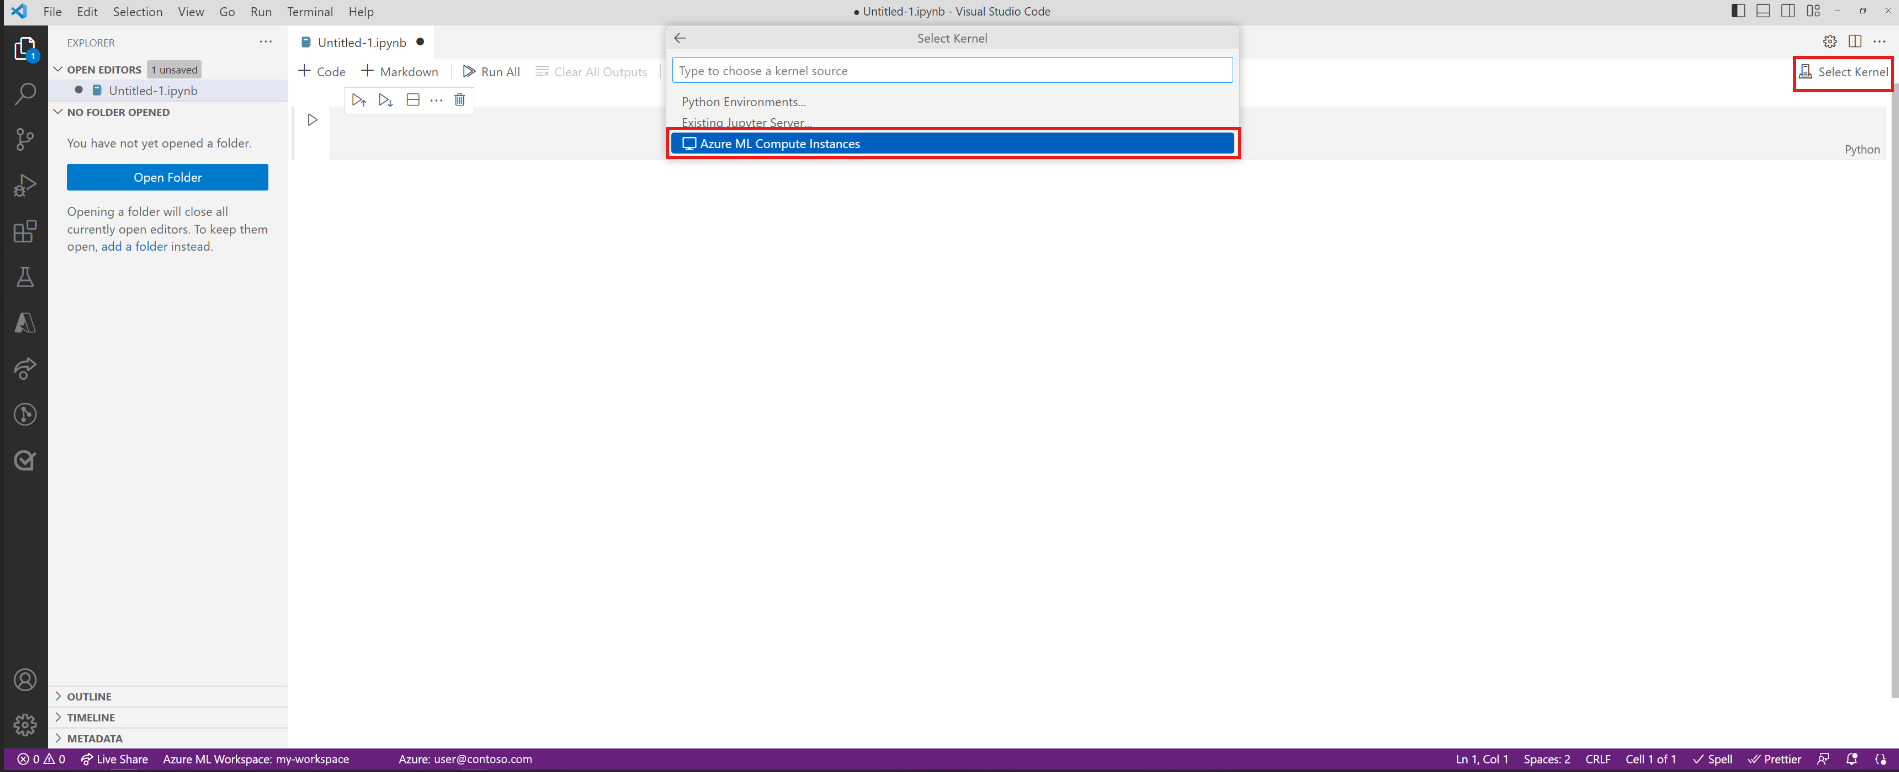
\includegraphics[scale = 0.3]{attachment/chapter_AML/Scc015}
	\caption{Kernel Selection in a Jupyter Notebook}
\end{figure}

In \gls{vsc}, there are multiple options to select a \gls{g_Kernel_Jy}. With the Azure ML extension, the option \textit{Azure ML Compute Instance} is available to.  On the compute instance, a variety of \gls{g_Kernel_Jy} are pre-installed.
\begin{figure}[H]
	\centering
	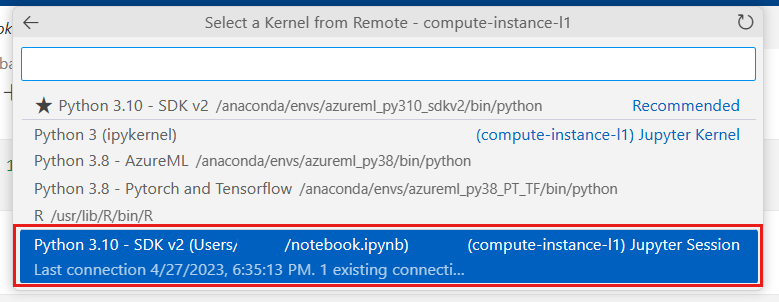
\includegraphics[scale = 0.3]{attachment/chapter_AML/Scc016}
	\caption{Kernel Sources}
\end{figure}

This connection allows to utilize the Azure ML Compute Instance, not all the other resource's. In the following the interaction between and to the other resources will be discussed.

\paragraph{Problem $\&$ Fix: Unable to connect}
One problem accrued. 
\begin{figure}[H]
	\centering
	
\includegraphics[scale = 0.3]{attachment/chapter_AML/Scc017}
	\caption{Error message after selecting Azure ML Compute Instance}
\end{figure}

For the moment, rollback the \gls{g_JupyterNotebook} extension to a version v2023.10.xxx helped.\footnote{
	\href{https://github.com/microsoft/vscode-jupyter/issues/14925}{Posted Problem}, \href{https://github.com/microsoft/vscode-jupyter/pull/14929}{Pull Request and Workaround}
}
\begin{figure}[H]
	\centering
	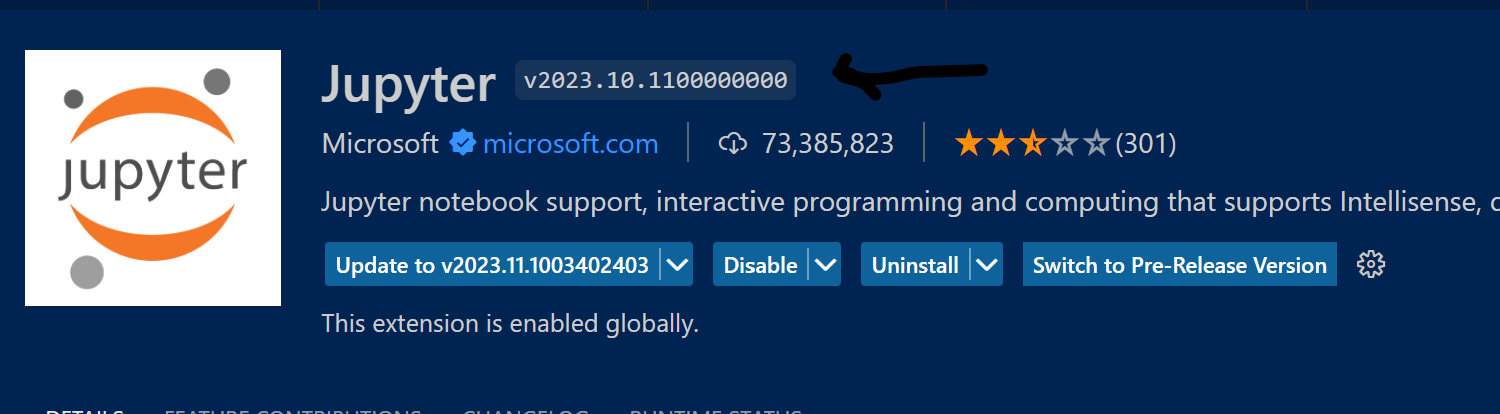
\includegraphics[scale = 0.3]{attachment/chapter_AML/Scc018}
	\caption{Rollback version}
\end{figure}

\subsubsection{Tunnel Connection}
\begin{comment}
	## Unclear, how this is going to work
	
	If a tunnel is made between \gls{vsc} and the the workspace the \gls{CLI} can be access by the terminal, see \href{https://learn.microsoft.com/de-de/azure/machine-learning/how-to-work-in-vs-code-remote?view=azureml-api-2}{Using az login --identity}
	
\end{comment}
With the option to connect to the workspace it self, the blobstorage, where the notebooks of each user are stored, can be access. To to this \gls{vsc} connected via tunnel to the workspace with the compute instance in the web browser or with the desktop application.
 
\begin{figure}[H]
	\centering
	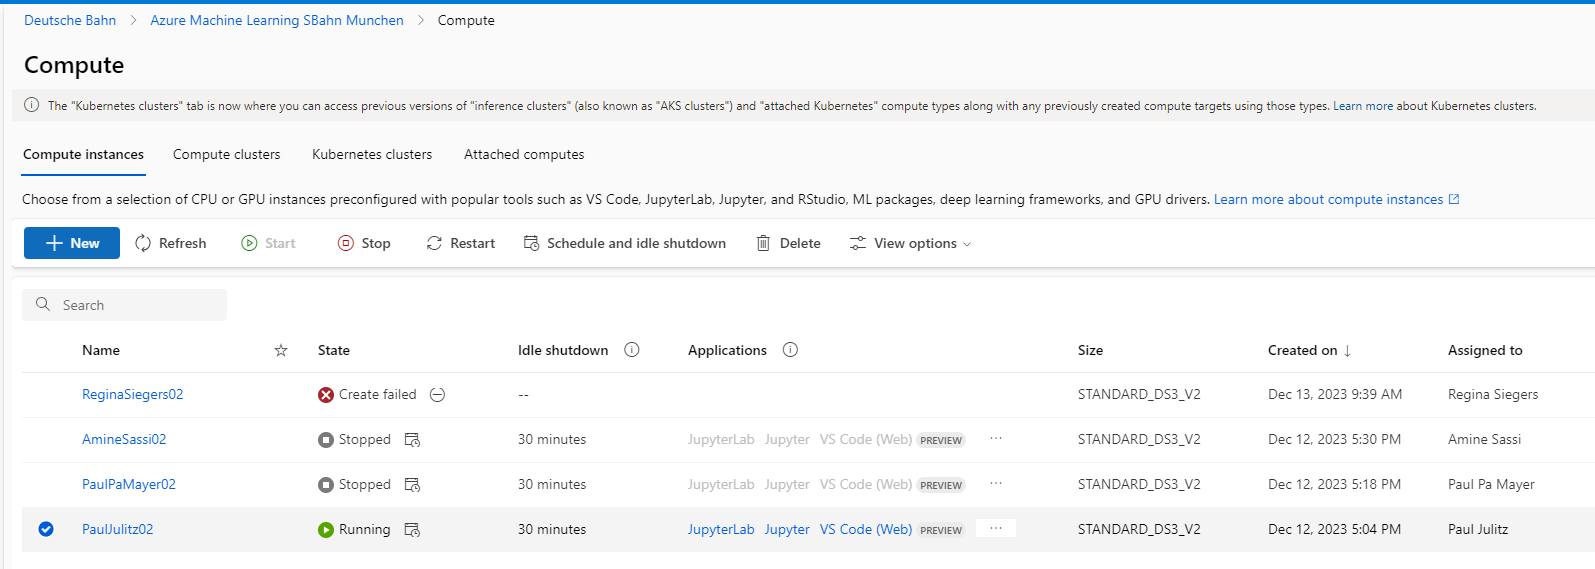
\includegraphics[scale = 0.3]{attachment/chapter_AML/Scc022}
	\caption{Create a tunnel connection}
\end{figure}

On the bottom left (1) the tunnel connection is displayed. The internal file system gets linked as the storage (2), where the notebook can be access. Note: Locally stored notebooks can be used by the previous section.

\begin{figure}[H]
	\centering
	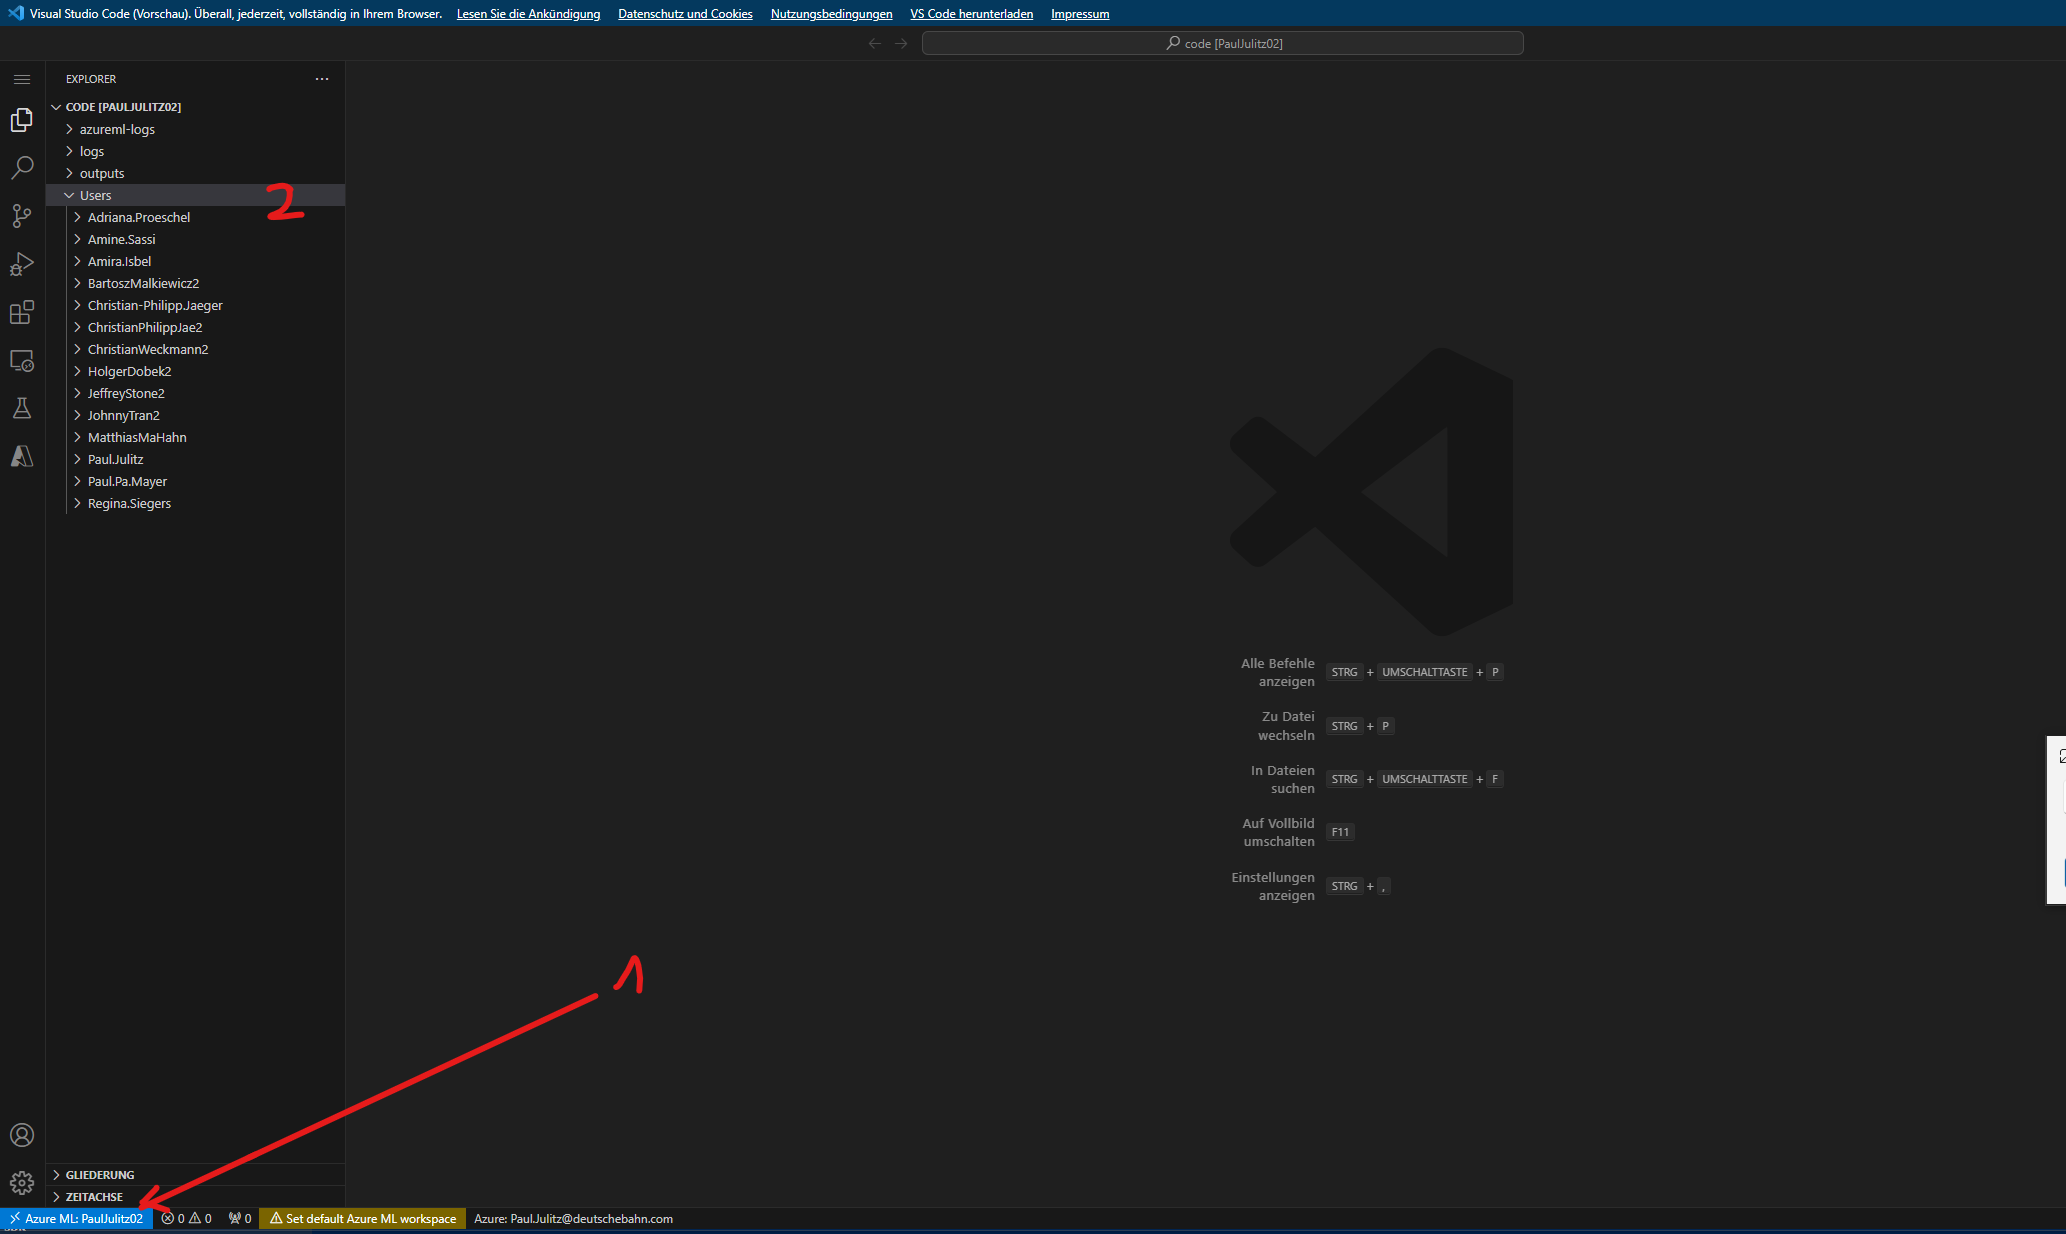
\includegraphics[scale = 0.3]{attachment/chapter_AML/Scc021}
	\caption{Create a tunnel connection}
\end{figure}


\subsection{Running WITH the Compute Instance (SDK v1)}

This section will explain how to use \gls{AML} with your local computer as a compute resources.
%\footnote{Reference: \href{https://learn.microsoft.com/en-us/azure/machine-learning/how-to-configure-environment?view=azureml-api-2#local-computer-or-remote-vm-environment}{Guide Installing SDK for Local Computer}}

%TODO: Setting Up a experiment, by using a compute instance 
%TODO: Setting up an experiemnt, by using local compute.
\subsubsection{Using a local kernel/ Python Interpreter}

\begin{itemize}
	\item Create a \gls{g_Python} \gls{VEN} with conda on you local computer
	\item Install the newest \gls{AMLSDKv1}.
	\footnote{
	Because the more extensive example is setup with \gls{AMLSDKv1}, we will start from here to. The idea is, that more functionally are provides by \gls{AMLSDKv2} then this will be incrementally be used. \href{https://learn.microsoft.com/en-us/python/api/overview/azure/ml/install?view=azure-ml-py}{Installation Guide}
}
	\begin{lstlisting}[style=CMD, caption={Installing Azure ML SDK core package},captionpos=b]
		pip install azureml-core
	\end{lstlisting}
	The \gls{SDK} contains many more optional packages, see \href{https://learn.microsoft.com/en-us/python/api/overview/azure/ml/install?view=azure-ml-py}{Optional Packages for Azure ML}
	\item Installing \gls{g_JupyterNotebook} required packages.
\end{itemize}

\begin{lstlisting}[style=CMD, caption={Installing Azure ML SDK core package},captionpos=b]
	conda 
\end{lstlisting}